\documentclass{article}
\setcounter{tocdepth}{4} %Required to insert paragraph in TOC
\setcounter{secnumdepth}{4} %Required to insert paragraph in TOC

\usepackage{graphicx} % Required for inserting images
\graphicspath{ {./img/} }

\usepackage{blindtext}
\usepackage{titlesec}
\usepackage[dvipsnames]{xcolor}
\usepackage{geometry}
\geometry{
	a4paper,
	total={170mm,257mm},
	left=25mm,
	top=20mm,
}

\usepackage{adjustbox}
\usepackage{amsmath}
\usepackage{amssymb}
\usepackage{cancel}
\usepackage{caption}
\usepackage{subcaption}
\usepackage{titlesec}
\usepackage{float}
\usepackage{enumitem}
\usepackage{hyperref}
\usepackage{makecell}

\setcounter{secnumdepth}{4}

\titleformat{\paragraph}
{\normalfont\normalsize\bfseries}{\theparagraph}{1em}{}
\titlespacing*{\paragraph}
{0pt}{3.25ex plus 1ex minus .2ex}{1.5ex plus .2ex}

\title{Appunti Ing Software}
\author{Mattia Robuschi Caprara}
\date{}

\definecolor{CoverGreen}{RGB}{255,121,0}

\begin{document}
	
	\begin{titlepage}
		
		\pagecolor{CoverGreen}
		
		\vspace{25 mm}
		\begin{center}
			\large
			{\color{black}\textbf{Mattia Robuschi Caprara}} 
		\end{center}
		
		\begin{center}
			\huge
			{\color{black}\textbf{Ingegneria del Software}}
		\end{center}
		
		\vspace{45 mm}
		
		\begin{figure}[h]
			\centering
			\adjustbox{cfbox=white 5pt 0cm}{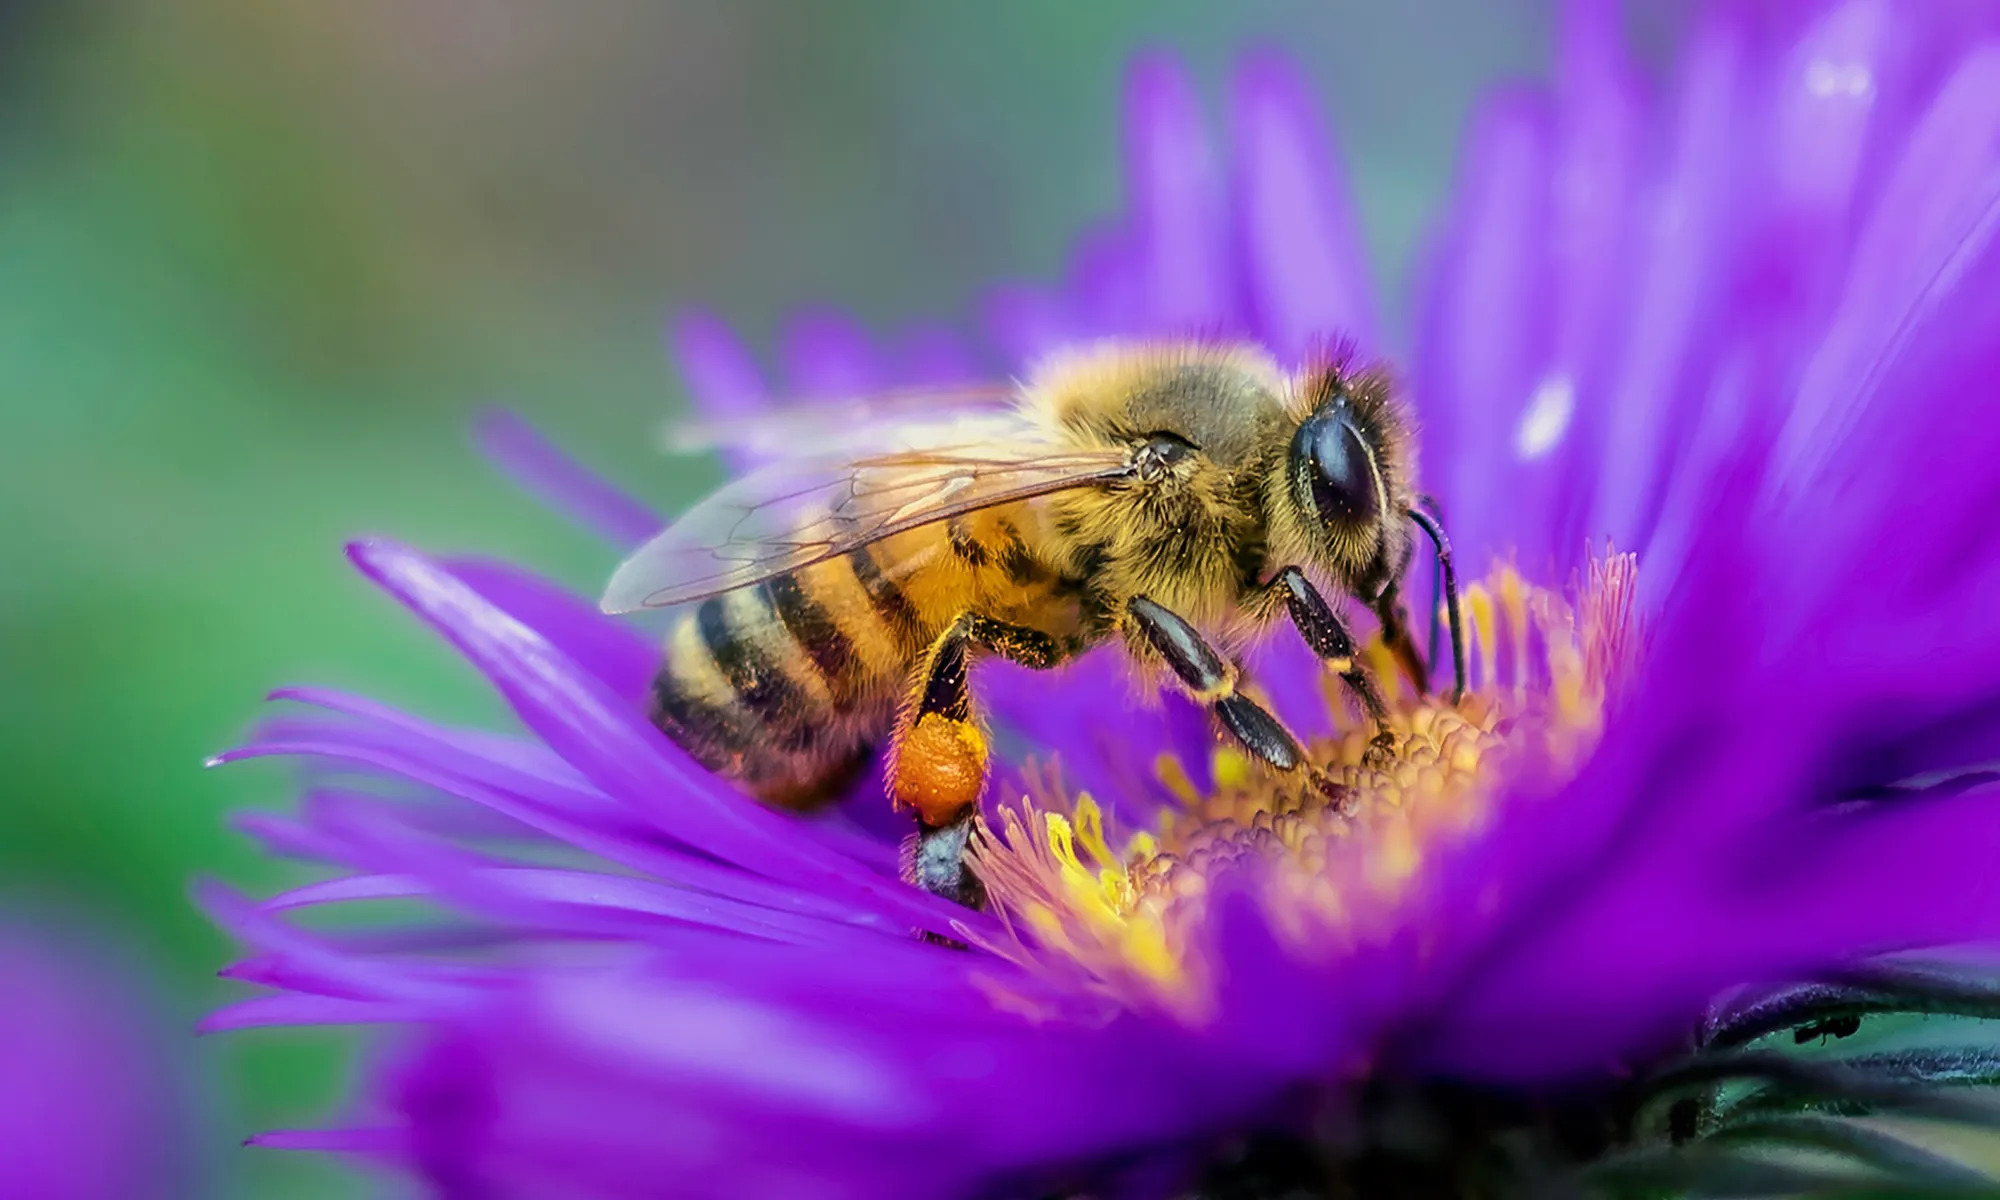
\includegraphics[scale=0.2]{0.cover.jpg}}
			%\caption{Caption}
			%\label{fig:enter-label}
		\end{figure}
		
		\thispagestyle{empty} 
	\end{titlepage}
	
	\newpage
	\pagecolor{white}
	\section*{Prefazione}
	Questi appunti sono una semplice riorganizzazione delle dispense fornite dal professor Agostino Poggi nell'anno accademico 2024/2025, di conseguenza alcune informazioni potrebbero essere troppo riassunte (Ad esempio: alcune sezioni sono solo delle semplici liste che illustrano nomi o temi ma senza approfondirne o spiegarne i significato, al contrario delle dispense) e potrebbe essere consigliato l'utilizzo di questi appunti insieme alle dispense del professore.
	\tableofcontents
	\newpage
	
	\section{Introduzione}
	\subsection{Caratteristiche e legami dell’ingegneria del software}
	Si basa su un insieme di tecniche, metodologie e strumenti. Ha l’obiettivo di produrre sistema software di alta qualità che soddisfano: il budget a disposizione, la data di scadenza del rilascio del sistema, e una corretta gestione dei cambiamenti che possono essere necessari durante lo sviluppo.
	\subsection{Ingegneria del Software e Risoluzione dei Problemi}
	\begin{enumerate}
		\item Fase di analisi: in cui si cerca di comprendere la natura del problema e di come suddividilo in parti.
		\item Fase di sintesi: in cui si Integrano tra loro le parti per ottenere
		il sistema finale.
	\end{enumerate}
	\subsection{Relazioni con Altre Discipline}
	Ha forti legami con:
	\begin{itemize}
		\item I linguaggi si programmazione
		\item I sistemi operativi
		\item Le basi di dati
		\item I modelli teorici
		\item L'intelligenza artificiale
		\item Le scienze organizzative
		\item L'ingegneria dei sistemi
	\end{itemize}
	\subsection{Particolarità del software}
	\begin{itemize}
		\item Il software è immateriale
		\item Il software richiede alta intensità umana
		\item Il software è malleabile
		\item Il software è complesso
		\item Il software è non Lineare
	\end{itemize}
	\subsection{Attività principali dell’Ingegneria del software}
	La realizzazione di sistemi software coinvolge cinque attività principali:
	\begin{itemize}
		\item Lo studio di fattibilità
		\item La definizione delle specifiche del software 
		\item Lo sviluppo del software
		\item La verifica del software
		\item L’evoluzione del software
	\end{itemize}
	\subsection{Proprietà del Software}
	Come tutti i tipi di sistemi, un sistema software deve garantire delle buone qualità e un corretto funzionamento. \\
	In particolare, il software di un sistema dovrebbe soddisfare un bel numero di proprietà:
	\begin{itemize}
		\item La correttezza
		\item L’affidabilità
		\item La robustezza
		\item Le prestazioni
		\item L’efficienza
		\item La scalabilità
		\item L’usabilità
		\item La verificabilità
		\item La manutenibilità
		\item La riusabilità
		\item La portabilità
		\item La comprensibilità
		\item L’ interoperabilità
		\item La produttività
		\item La tempestività
		\item La trasparenza
	\end{itemize}
	\subsection{Capacità necessarie per lo sviluppo di software}
	Lo sviluppo di un sistema software richiede le più diverse attività e capacità: 
	\begin{itemize}
		\item Risolvere dei problemi
		\item Acquisire delle conoscenze
		\item Prendere delle decisioni
		\item Astrarre oggetti e sistemi
		\item Definire dei modelli
		\item etc.
	\end{itemize}
	\subsection{Capacità e Conoscenze dell’Ingegnere del software}
	Un ingegnere del software deve essere: 
	\begin{itemize}
		\item Un buon programmatore
		\item Un esperto in strutture dati e algoritmi 
		\item Un esperto in uno o più linguaggi di programmazione
		\item Familiare con le differenti aree applicative e con più approcci di progettazione
		\item Capace a muoversi tra i diversi livelli di astrazione di un progetto
		\item Capace di costruire diverse varietà di modelli
		\item In grado di fare scelte tra le possibili soluzioni disponibili
		\item In grado di comunicare e interagire con le persone
		\item In grado di tradurre descrizioni e risposte (in genere del cliente) anche vaghe in precise specifiche.
	\end{itemize}
	\subsection{Ruoli nello sviluppo del software}
	\begin{itemize}
		\item Il cliente
		\item Il manager (Gestore del progetto)
		\item L'analista
		\item Il programmatore
		\item Il gestore dei test
		\item Il consulente
		\item L'utente
	\end{itemize}
	\subsection{Responsabilità professionale ed etica}
	L'ingegneria del software comporta responsabilità più ampie rispetto alla
	semplice applicazione di competenze tecniche.\\
	Ogni persona coinvolta in un progetto dovrebbe: comportarsi in modo onesto ed eticamente
	responsabile e offrire competenza e riservatezza.
	\subsection{Sistemi software}
	Sono dei sistemi che utilizzano componenti, hardware e software e hanno come obiettivo principale quello di soddisfare le esigenze del cliente.\\
	Un sistema software di successo può rimanere in servizio per
	parecchi anni e, durante la sua vita, può subire numerose modifiche e
	estensioni.
	\subsection{Stima dei Costi del Software}
	Due tipi di metriche:
	\begin{itemize}
		\item Dimensionali: in cui la stima del costo di basa sul numero
		di linee di codice prodotte, Il numero di istruzioni in ‘’linguaggio macchina’’
		e Il numero di pagine di documentazione del sistema.
		\item Funzionali: in cui la stima del costo si basa sui numeri di
		classi, attributi, relazioni, metodi, messaggi, parametri dei messaggi,
		sorgenti e destinazioni dei messaggi, la percentuale di riuso, il numero
		di oggetti, la complessità di ciascun oggetto e la produttività.
	\end{itemize}
	\begin{figure}[h]
		\centering
		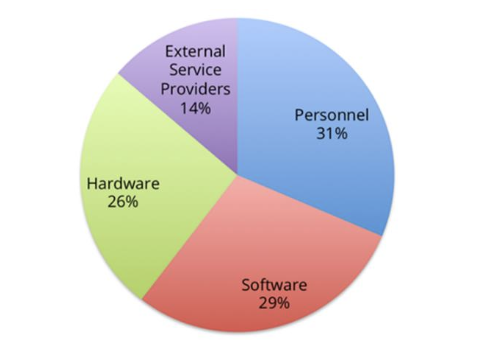
\includegraphics[scale=0.8]{1.dist_costi.png}
		\caption{Distribuzione dei costi di sviluppo sistema software}
		%\label{fig:enter-label}
	\end{figure}
	\subsection{Dominio applicativo o del problema}
	In ingegneria del software e in altre discipline informatiche, per dominio applicativo (o dominio del problema) s'intende il contesto in cui opera un'applicazione.\\
	Per limitare i problemi dello sviluppo di un sistema è necessario avere delle buone conoscenze del suo dominio applicativo.\\
	Queste conoscenze possono essere identificate tramite \textbf{l'analisi del dominio}.\\
	Quest’analisi ha l’obiettivo di comprendere a fondo i concetti, le dinamiche, le regole generali che definiscono il dominio applicativo in cui il sistema software dovrà essere impiegato.\\
	La qualità dei risultati dipende dal tipo di persone coinvolte, oltre a degli analisti sono coinvolti anche esperti del dominio in questione.
	\subsection{Ciclo di vita di un sistema software}
	Il ciclo di vita di un sistema software coinvolge in genere 5 attività
	principali:
	\begin{enumerate}
		\item L’analisi preliminare
		\item La progettazione
		\item La realizzazione
		\item La gestione
		\item La messa fuori servizio del sistema
	\end{enumerate}
	\subsection{Difficoltà dello sviluppo del software}
	Con il passare del tempo, l’evoluzione delle tecnologie software permette lo sviluppo di sistemi sempre più complessi e quindi i sistemi che si vogliono realizzare richiedono nuove competenze e capacità.\\
	Il processo di sviluppo di un sistema software è difficile da gestire, Questo è dovuto in parte al fatto che il software offre un'\textbf{estrema flessibilità} ed è un \textbf{sistema discreto}.\\
	Per estremamente flessibile si intende che il software è modificabile con pochissimo sforzo, ma ciò incoraggia un modo di lavorare non pianificato, che può essere un rischio.\\
	La non linearità fa sì che un piccolo cambiamento nel codice può portare a grandi cambiamenti (spesso indesiderati) nel funzionamento di un’applicazione.\\
	Le difficoltà nel realizzare un sistema software sono spesso aumentate dagli obiettivi e dalle richieste degli stakeholder.
	\subsection{Richieste più frequenti}
	Sono frequenti le richieste di aggiunta e/o modifica di parti del sistema e le richieste di riduzione dei tempi la consegna.\\
	I risultati dipendono dal peso (tempo in meno e lavora da fare) delle richieste.
	\subsection{Problemi tipici}
	\begin{itemize}
		\item Consegna del sistema ritardata
		\item Sforamento del budget
		\item Bassa affidabilità
		\item Basse prestazioni del sistema
		\item Difficoltà nella manutenzione del sistema
		\item Difficoltà nell’aggiunta di funzionalità al sistema.
	\end{itemize}
	Nel caso di sistemi molto complessi, la presenza di diversi risultati negativi può precedere un’elevata probabilità di ritiro del progetto di sviluppo.
	\subsection{Sfide dell’Ingegneria del software}
	Il successo dell’ingegneria del software per sviluppare sistemi non solo utili, ma anche molto utilizzati può essere aiutato attraverso la valorizzazioni di alcune proprietà:
	\begin{itemize}
		\item Eterogeneità: la capacità di realizzare sistemi integrando diversi tipi di software e/o hardware
		\item Cambiamento sociale: comporta un mutamento significativo della società dovuto in gran parte dallo sviluppo tecnologico che offre sempre nuovi interessi
		\item Sicurezza e Fiducia: due componenti che permettono a un cliente
		e/o utente di valutare, in modo positivo o negativo, la possibilità di fare
		delle scelte.
		\item Evoluzione tecnologica
	\end{itemize}
	\subsection{Stakeholder}
	Gli stakeholder sono tutte le persone che in qualche modo sono interessate allo sviluppo di un sistema.\\
	Queste persone possono essere:
	\begin{itemize}
		\item Ingegneri
		\item Programmatori
		\item Manager aziendali
		\item Esperti di dominio
		\item Rappresentanti sindacali
		\item Utenti finali
		\item Tutti i membri di un'organizzazione che potrebbero essere interessati all'installazione del sistema software
	\end{itemize}
	\subsection{Obiettivi degli Stakeholder}
	Gli stakeholder hanno spesso interessi e obiettivi diversi che in genere dipendono dal ruolo che giocano nel progetto.\\
	\begin{table}[h!]
		\centering
		\begin{tabular}{ |c|c|c| } 
			\hline
			\textbf{Stakeholder} & \textbf{Interesse nel progetto}\\
			\hline
			Sviluppatori & Elevata produttività, prevenzione degli errori,
			poche rilavorazioni\\
			\hline
			Venditori & Cifre di vendita elevate, maggiore soddisfazione del cliente\\
			\hline
			Responsabili del progetto & Riduzione del budget, rispetto del programma\\
			\hline
			Investitori & Time-to-market più breve, flussi di lavoro più rapidi\\
			\hline
			Clienti e Utenti & Flusso di lavoro più semplice, buona usabilità\\
			\hline
		\end{tabular}
		\caption{Stakeholders e i loro interessi}
	\end{table}

	\subsection{Tipi di sistema software}
	I metodi e gli strumenti di ingegneria del software utilizzati dipendono da: il tipo di
	applicazione sviluppata, i requisiti del cliente e il background del team di sviluppo.\\
	Tipi di sistema software:
	\begin{itemize}
		\item Sistemi autonomi
		\item Sistemi interattivi
		\item Sistemi di controllo integrati (Embedded Control Systems)
		\item Sistemi di elaborazione batch
		\item Sistemi di intrattenimento
		\item Sistemi per la modellazione e simulazione
		\item Sistemi di raccolta dati (Data Collection Systems)
		\item Sistemi di sistemi (Systems of Systems)
	\end{itemize}
	
	\section{Attività software di base}
	\subsection{Proprietà del Buon Software}
	\subsection{Legge sugli Standard di Ambler}
	\begin{figure}[h]
		\centering
		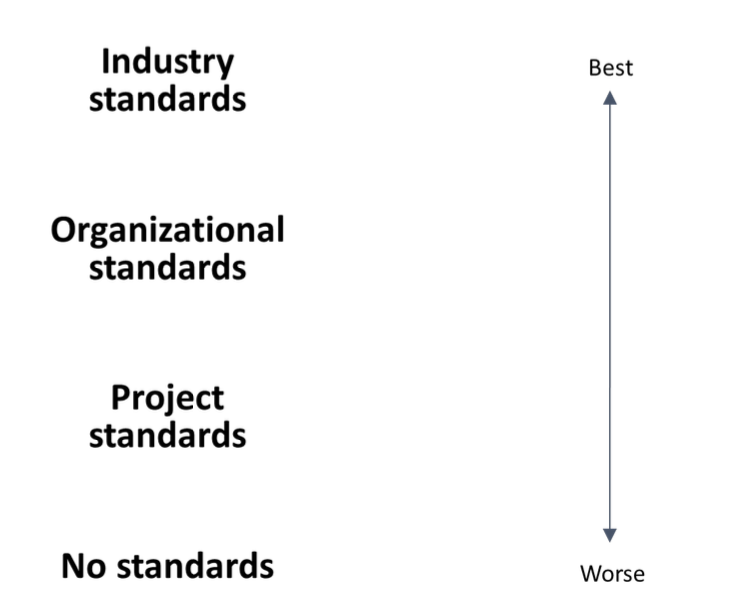
\includegraphics[scale=0.3]{2.qual_stili.png}
		\caption{Livelli di qualità degli stili}
		%\label{fig:enter-label}
	\end{figure}
	\begin{figure}[h]
		\centering
		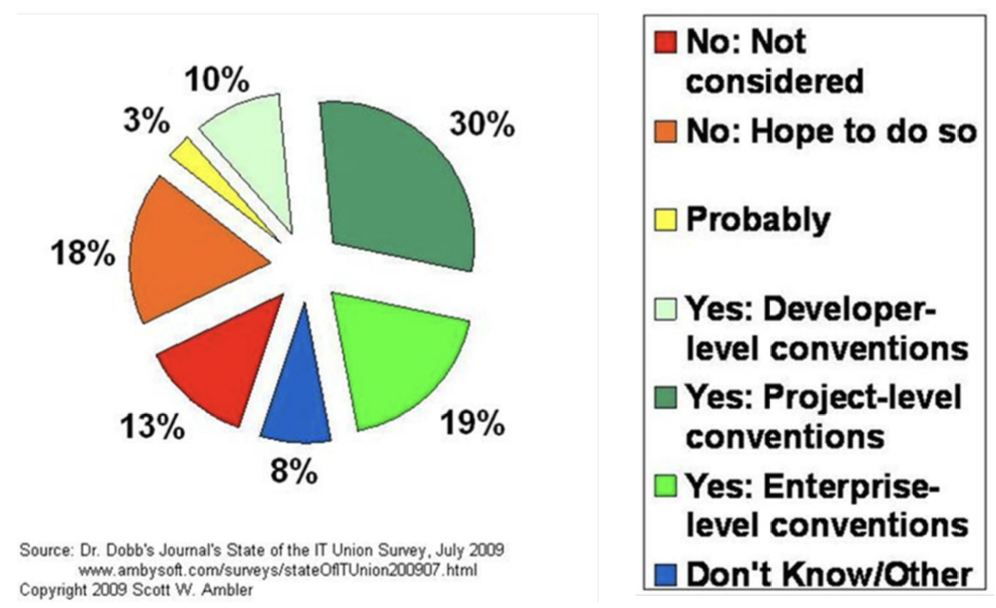
\includegraphics[scale=0.3]{3.diff_stili.png}
		\caption{Diffusione dell'uso degli stili}
		%\label{fig:enter-label}
	\end{figure}
	\subsection{Convenzioni di Codifica dei Nomi}
	\subsection{Gestione degli Errori}
	\subsection{Distribuzione Statistica degli Errori}
	\subsection{Fonti degli Errori}
	\subsection{Difficoltà nel Riconoscere gli Errori}
	\subsection{Passi per Correggere un Errore}
	\subsection{Uso di Istruzioni di Stampa}
	\subsection{Strumenti a Supporto della Correzione di Errori}
	\subsection{Tecniche Principali di Analisi Statica}
	\subsection{Testing}
	
	\section{Processi software}
	\subsection{Processi e modelli di processi software}
	Plan driven
	Agili
	\subsection{Studio di fattibilità}
	\subsection{Modello a cascata}
	Problemi del modello a cascata
	\begin{figure}[h]
		\centering
		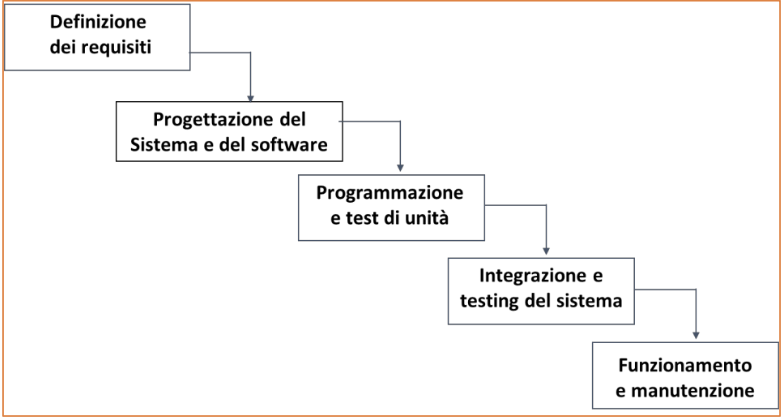
\includegraphics[scale=0.3]{4.mod_cascata.png}
		\caption{Schema funzionamento modello a cascata}
		%\label{fig:enter-label}
	\end{figure}
	Applicabilità del Modello a Cascata
	Modello a Cascata – Pro e Contro
	Modello a cascata con feedback
	\begin{figure}[h]
	\centering
	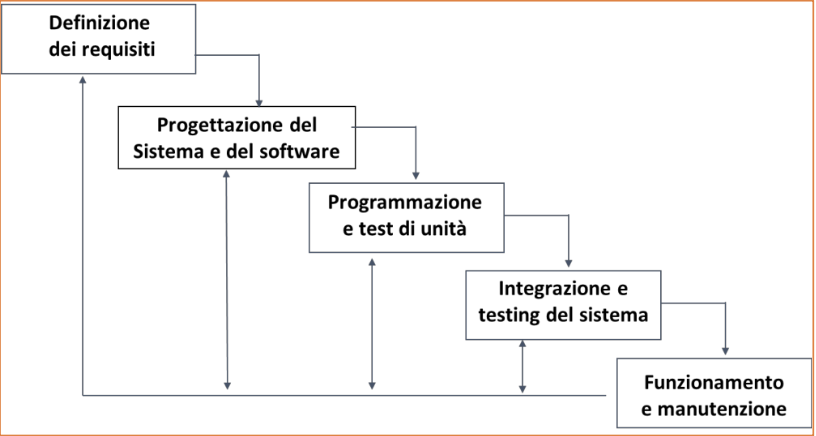
\includegraphics[scale=0.3]{5.mod_cascata_fb.png}
	\caption{Schema funzionamento modello a cascata con feedback}
	%\label{fig:enter-label}
	\end{figure}
	Ad ogni step posso tornare ai precedenti
	Waterfall V Model
	\begin{figure}[h]
		\centering
		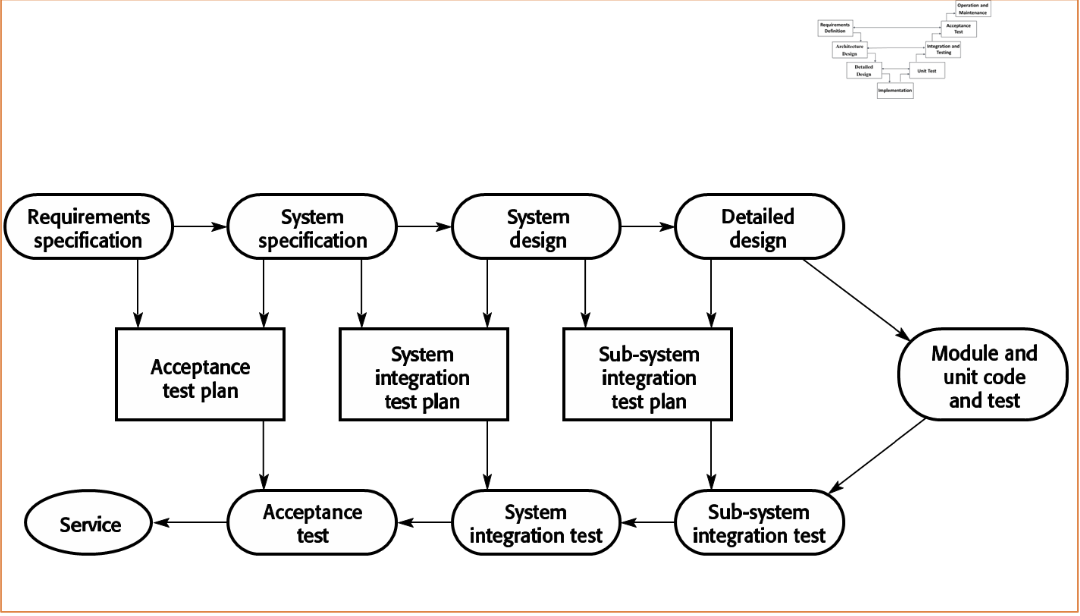
\includegraphics[scale=0.3]{6.mod_cascata_v.png}
		\caption{Schema funzionamento modello a cascata V}
		%\label{fig:enter-label}
	\end{figure}
	Associazione di una fase di testing per ogni fase di sviluppo
	\subsection{Modello Sviluppo Incrementale - Sviluppo Incrementale}
	\begin{figure}[h]
		\centering
		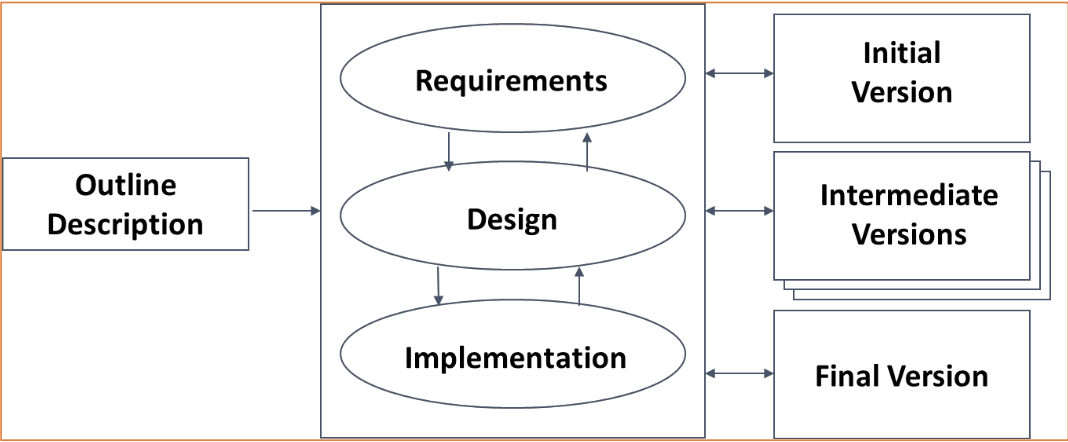
\includegraphics[scale=0.3]{7.svil_inc.png}
		\caption{Schema funzionamento sviluppo incrementale}
		%\label{fig:enter-label}
	\end{figure}
	Suddivisione in incrementi
	Sviluppo e consegna incrementale – Pro e Contro
	Applicabilità dello sviluppo incrementale
	\begin{figure}[h]
		\centering
		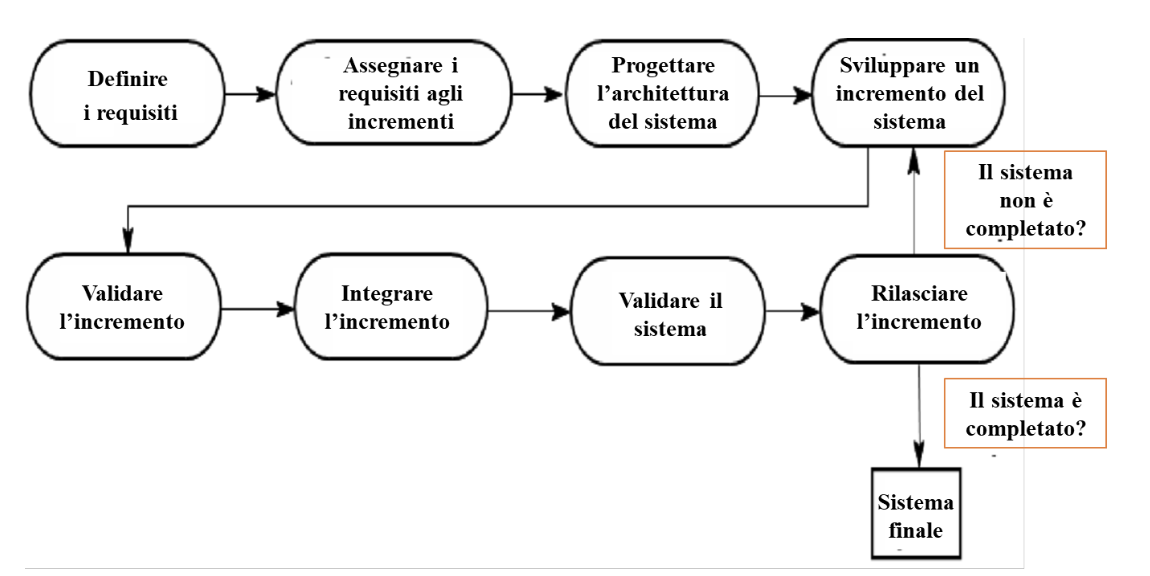
\includegraphics[scale=0.3]{8.diag_svil_inc.png}
		\caption{Diagramma funzionamento sviluppo incrementale}
		%\label{fig:enter-label}
	\end{figure}
	\subsection{Modello Integrazione e Configurazione}
	Basato sul riutilizzo del software (componenti, libs, ecc…)
	\begin{figure}[h]
		\centering
		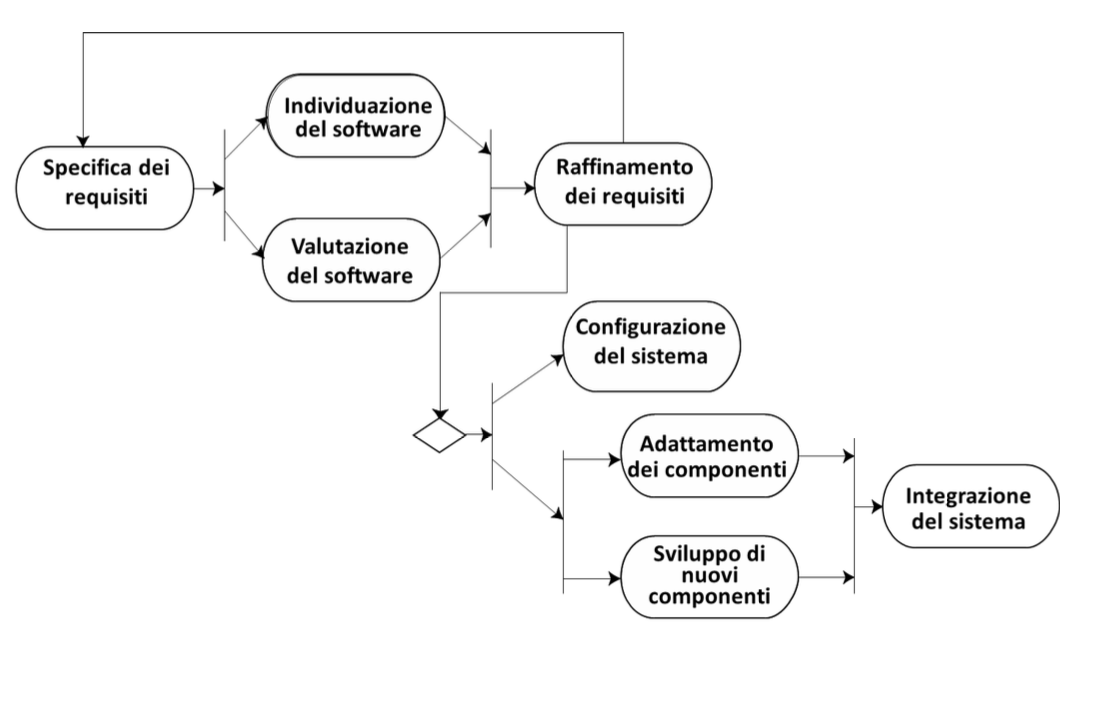
\includegraphics[scale=0.3]{9.diag_int_conf.png}
		\caption{Diagramma funzionamento Integrazione e configurazione}
		%\label{fig:enter-label}
	\end{figure}
	Integrazione e Configurazione – Pro e Contro
	\subsection{Distribuzione dei Costi di Sviluppo}
	\begin{figure}[h]
		\centering
		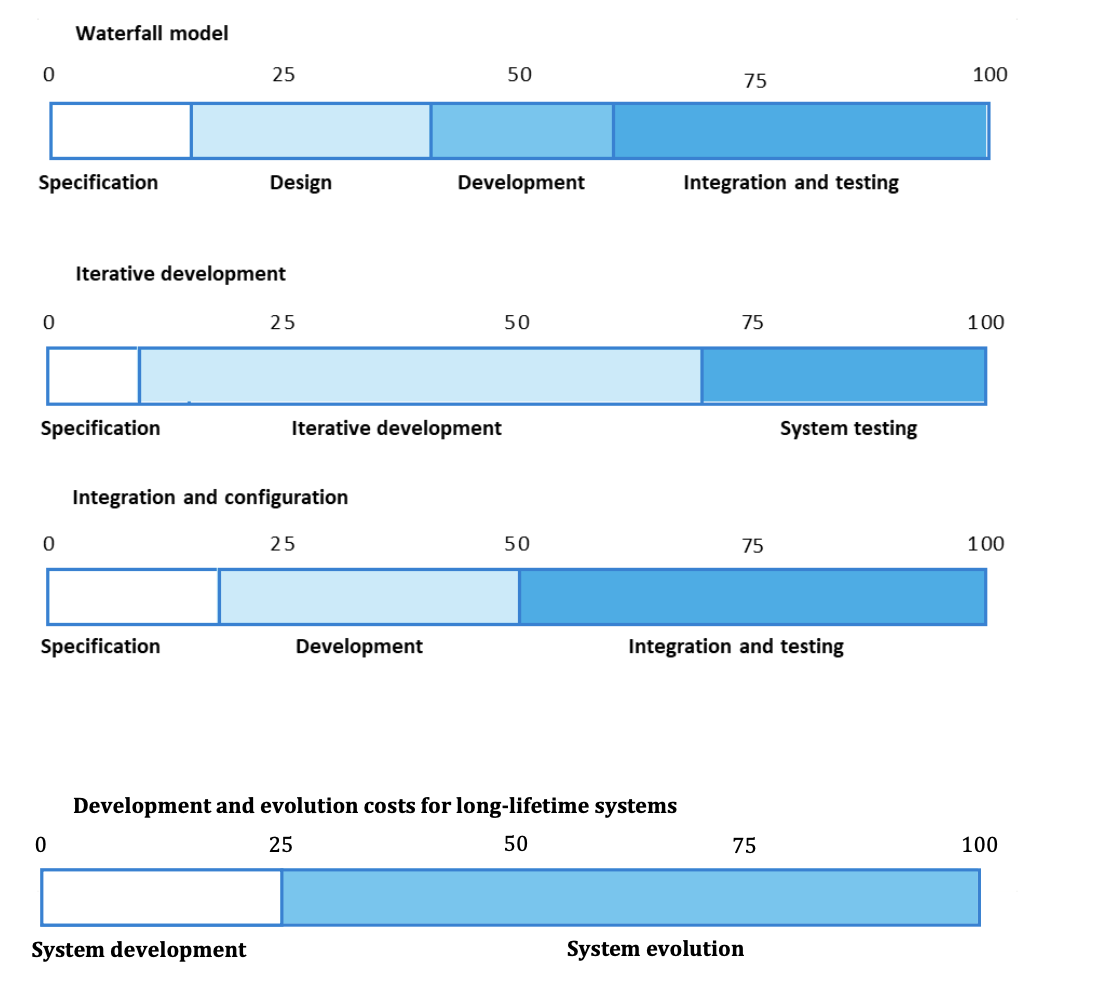
\includegraphics[scale=0.3]{10.dist_cost_svil.png}
		\caption{Grafico distribuzione costi di sviluppo}
		%\label{fig:enter-label}
	\end{figure}
	
	\section{Ingegneria dei requisiti}
	\subsection{Definizione di Ingegneria dei Requisiti}
	\subsection{Definizione e astrazione dei requisiti}
	\subsection{Requisiti dell’Utente e del Sistema}
	\subsection{Imprecisione dei Requisiti}
	\subsection{Consistenza e Complessità dei Requisiti}
	\subsection{Tipi di Requisiti}
	Funzionali
	Funzionalità e servizi che il sistema deve fornire
	Non funzionali
	Proprietà e vincoli del sistema
	Di dominio
	\subsection{Classificazione dei Requisiti non Funzionali}
	Requisiti del prodotto
	Requisiti organizzativi
	Requisiti esterni
	\begin{figure}[h]
		\centering
		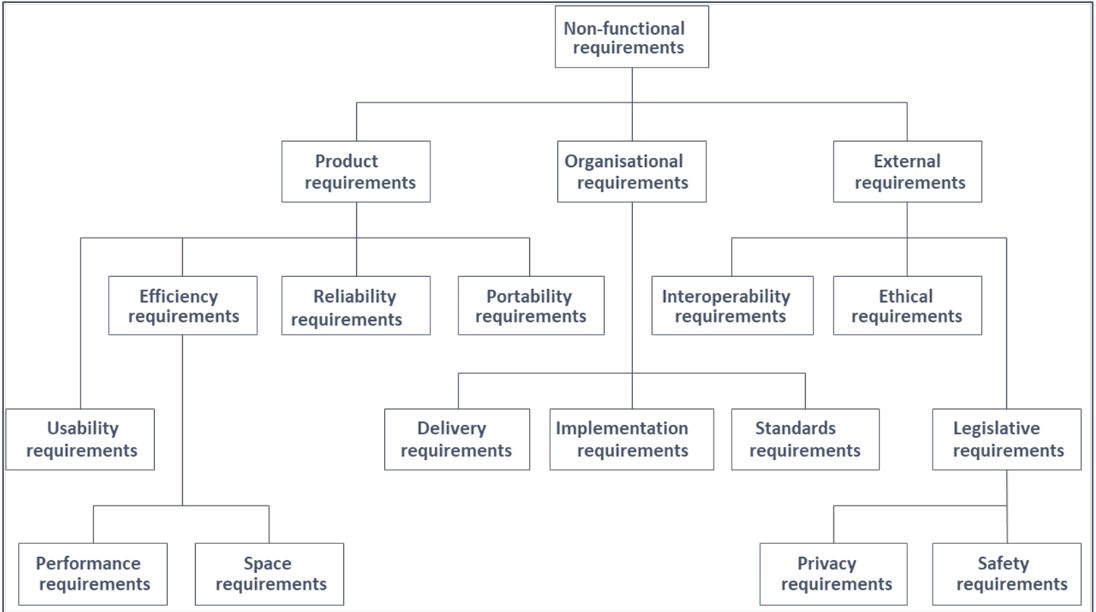
\includegraphics[scale=0.3]{11.tipi_ric_non_func.png}
		\caption{Tipologie dei requisiti non funzionali}
		%\label{fig:enter-label}
	\end{figure}
	Obiettivi e Requisiti non Funzionali Verificabili
	\begin{table}[h!]
		\centering
		\begin{tabular}{ |c|c|c| } 
			\hline
			\textbf{Proprietà} & \textbf{Misure}\\
			\hline
			Velocità & \makecell{Transazioni elaborate/secondo \\ Tempo di risposta utente/evento \\ Tempo di aggiornamento dello}\\
			\hline
			Dimensioni & \makecell{Gbyte \\ Numero di chip ROM}\\
			\hline
			Facilità d'uso & \makecell{Tempo di allenamento \\ Numero di frame di aiuto}\\
			\hline
			Affidabilità & \makecell{Tempo medio al fallimento \\ Probabilità di indisponibilità \\ Tasso di occorrenza del guasto Disponibilità}\\
			\hline
			Robustezza & \makecell{Tempo necessario per riavviare dopo il fallimento \\ Percentuale di eventi che causano guasti \\ Probabilità di danneggiamento dei dati in caso di errore}\\
			\hline
			Portabilità & \makecell{Percentuale di istruzioni dipendenti dall'implementazione \\ Numero di parti/componenti da "studiare"}\\
			\hline
		\end{tabular}
		\caption{Esempi di metriche per i requisiti non funzionali}
	\end{table}
	\subsection{Processi dell’Ingegneria dei Requisiti}
	Raccolta (Elicitazione)
	Analisi
	Convalida
	Gestione
	Processo Base dell’Ingegneria dei Requisiti
	Processo dell’Ingegneria dei Requisiti a Spirale
	\subsection{Raccolta dei Requisiti e relativi problemi}
	Tecniche di Raccolta dei Requisiti
	Interviste
	Questionari
	Brain Storming
	Etnografia (Osservazione degli utenti)
	Integrazione dell’Etnografia con la Prototipazione
	\subsection{Specifica dei Requisiti}
	Linee Guida per la Descrizione dei Requisiti
	Dettagia requisiti utente e requisiti di sistema
	Strumenti per la Descrizione dei Requisiti
	Requisiti di una Pompa per Insulina
	\subsection{Specifiche Basate sui Moduli}
	Specifica Modulare della Dose di Insulina
	\subsection{Specifiche Tabulari}
	Specifica Tabulare della Dose di Insulina
	\subsection{Documento dei Requisiti del Software}
	Variabilità e problemi dei Documenti dei Requisiti
	Verifica dei Requisiti
	Tecniche per la Verifica dei Requisiti
	Domande di Controllo della Revisione
	\subsection{Gestione dei Requisiti}
	Elementi a Supporto della Gestione dei Requisiti
	\subsection{Modifica dei Requisiti}
	Processo di Gestione dei Cambiamenti (Semplificato) \\
	Processo di Gestione dei Cambiamenti (Dettagliato)
	\subsection{Tracciabilità}
	Esempi di Documenti di Tracciabilità
	
	\section{Sviluppo di software agile}
	\subsection{Metodologia Agile}
	Caratteristiche principali dello sviluppo agile
	Sviluppo e rilascio rapido del software
	\subsection{Extreme programming (XP)}
	Requisiti espressi come user stories
	XP and Principi del Metodo Agile
	XP \& Storie degli Utenti
	Diagramma – Ciclo di Sviluppo XP
	\subsection{Sviluppo guidato dai test}
	\subsection{Programmazione a coppie}
	\subsection{Metodi agili e manutenzione del software}
	Problemi della manutenzione agile
	\subsection{Scelta tra metodi agili e guidati dai piani}
	\subsection{Coinvolgimento del Cliente}
	\subsection{Automazione dei Test}
	Problemi dello Sviluppo basato sui Test
	5\subsection{Refactoring}
	Costante miglioramento del codice
	Esempi di Refactoring
	Principi di refactoring
	\subsection{Problemi pratici dei metodi agili}
	\subsection{Metodi agili e manutenzione del software}
	\subsection{Problemi contrattuali}
	\subsection{Problemi organizzativi}
	\subsection{Gestione agile dei progetti}
	\subsection{Scrum}
	Basato su sprint, periodi di tempo in cui il team sviluppa e completa una determinata quantità di lavoro
	Diagramma del Ciclo di Sprint
	Benefici dell’uso di Scrum
	\subsection{Scalabilità dei metodi agili}
	Scalabilità verticale e orizzontale
	Verticale: metodi agili che non possono essere integrati in software di grandi dimensioni
	Orizzontale: metodi agili che possono essere integrati in una grande organizzazione
	Sviluppo di sistemi di grossa dimensione
	Scalabilità verticale di grossi sistemi
	
	\section{Modelli dei sistemi e UML}
	\subsection{Modellazione del Sistema}
	\subsection{Tipi di Modelli}
	Modelli pedittivi
	Modelli estrattivi
	Modelli prescrittivi
	\subsection{Prospettive dei Sistemi Software}
	\subsection{Riuso e attività nell’ambito dei modelli}
	\subsection{Attività nell’Ambito dei Modelli}
	\subsection{UML}
	Motivi del Successo di UML
	Viste di UML
	Tipi di Diagrammi UML
	Use Case Diagram
	Structural View Diagram
	Implementation View Diagram
	Enviroment View Diagram
	Behavioral View Diagram
	Statistica dell’Uso dei Diagrammi
	\subsection{Proprietà ed elementi dei diagrammi dei casi d’uso}
	Elementi dei Casi di Uso
	Boundary
	Attori
	Casi d’uso
	Esempio di caso di uso
	Connettori e Valori di Molteplicità
	\subsection{Classi, interfacce e modificatori}
	Modelli di Classe a Diverso Livello di Dettaglio
	Associazione
	Semplice associazione fra classi, definise le regole per le altre associazioni
	Generalizzazione, Nesting, Dipendenza e Realizzazione
	Generalizzazione: Indica ereditarietà, freccia che va dalla SubClass alla SuperClass
	Nesting: Elemento di origine dentro alla classe
	Dipendenza: forma debole di relazione
	Realizzazione: Indica la realizzazione di un’interfaccia
	Aggregazione e Composizione
	Aggregazione: La/le classe/i è contenuta all’interno di un’altra classe (Rombo vuoto)
	Composizione: Le classi compongono una classe più grande (es. albero composto da foglie, rami, tronco, radici, ecc…) (Rombo pieno)
	\subsection{Diagramma di Sequenza}
	Lifeline
	Elementi del diagramma di sequenza
	Messaggi usati nel diagramma di sequenza
	\subsection{Diagramma delle Attività}
	Esempio di Diagramma delle Attività
	Tipi di Nodi di Controllo
	Input \& Output Pins
	Decisioni
	Concorrenza
	Attività di Raggruppamento
	Timeout \& Signal
	\subsection{Diagramma degli Stati}
	Esempio di Diagramma degli Stati
	Pseudo-stato di Scelta e di Giunzione
	Stato Composto
	Storie dello Stato e Regioni Concorrenti
	\subsection{Diagramma degli Oggetti}
	Esempio di Diagramma degli Oggetti
	\subsection{Diagramma dei Componenti}
	Esempio di Diagramma dei Componenti
	\subsection{Diagramma delle Strutture Composite}
	Esempio di Diagramma delle Strutture Composite
	\subsection{Diagramma dei Package}
	Esempio di Diagramma dei Package
	\subsection{Diagramma di Comunicazione}
	Esempio di Diagramma di Comunicazione
	\subsection{Diagramma di Temporizzazione}
	Esempio del Diagramma di Temporizzazione
	\subsection{Diagramma di Panoramica dell’Interazione}
	Esempio di Diagramma di Panoramica dell’Interazione
	\subsection{Diagramma di Distribuzione}
	Relazioni fra hardware e software
	Esempio di Diagramma di Distribuzione
	\subsection{Diagramma di Robustezza}
	Tipi di Nodi
	Boundary
	Control
	Entity
	Diagramma di robustezza e comunicazione
	Diagramma di robustezza e sequenza
	\subsection{Tool per il disegno di diagrammi UML}
	Eclipse Papyrus e app.diagrams.net
	
	\section{Modelli e Classi di Analisi}
	\subsection{Modello di analisi dei requisiti}
	\subsection{Modello di analisi orientati agli oggetti}
	\subsection{Classi di analisi}
	\subsection{Categorie delle classi di analisi}
	\subsection{Tecniche di individuazione delle classi}
	Analisi nome – verbo
	\begin{table}[h!]
		\centering
		\begin{tabular}{ |c|c|c| } 
			\hline
			\textbf{Componente del testo} & \textbf{Modello del componente} & \textbf{Esempio}\\
			\hline
			Nome proprio & Istanza & Jim Smith\\
			\hline
			Nome comune & Classe &Giocattolo, bambola\\
			\hline
			Verbo di fare & Metodo & Comprare, consigliare\\
			\hline
			Verbo di classificazione & Eredità & è un\\
			\hline
			Verbo di possessione & Aggregazione & Ha un\\
			\hline
			Verbo modale & Vincolo & Deve essere\\
			\hline
			Aggettivo & Attributo & Di tre anni\\
			\hline
			Verbo transitivo & Metodo & Entra, modifica\\
			\hline
			Verbo intransitivo & Metodo (evento) & Dipende da\\
			\hline
		\end{tabular}
		\caption{Schema analisi nome-verbo}
	\end{table}
	Approccio guidato dai casi di uso
	Modelli di classi comuni
	Classi, responsabilità e collaborazioni (CRC)
	Approccio Misto
	\subsection{Errori Comuni di Analisi}
	\subsection{Diagramma delle Classi: Descrizione di un appartamento}
	\subsection{Diagramma delle Classi: Prenotazioni Online}
	\subsection{Diagramma delle Classi: Offerta formativa di una Università}
	
	\section{Scenari e casi d’uso}
	\subsection{Storie e scenari}
	\subsection{Casi di uso}
	Ranking dei casi di uso
	Operazioni principali dei casi di uso
	Guide per lo sviluppo dei casi di uso
	\subsection{Casi di Uso - Un Negozio di Vendita Online}
	\subsection{Casi di uso - Un altro negozio di vendita online}
	\subsection{Descrizione del Caso di Uso: Inserisci l’Ordine}
	Attori, Trigger, PreCondizioni e PostCondizioni
	Flusso Principale
	Flusso Alternativo 1
	Flusso Alternativo 2
	Flusso Alternativo 3
	\subsection{Template per i casi di uso}
	
	\section{Elementi di progettazione}
	\subsection{Processo di Progettazione}
	\subsection{Concetti e Principi di Progettazione}
	\subsection{Modularità}
	Difficoltà ad Individuare la Migliore Modularità
	\subsection{Coesione}
	\subsection{Accoppiamento}
	
	\section{Progettazione architetturale}
	\subsection{Scopo della Progettazione Architetturale}
	\subsection{Requisiti e Progettazione}
	\subsection{Diagrammi a Blocchi}
	\subsection{Astrazione Architetturale}
	\subsection{Progettazione dell’Architettura e Riuso}
	\subsection{Pattern Architetturali}
	Architettura - Model-View-Controller (MVC)
	Architettura - Layered
	Architettura - Repository
	Architettura - Pipe \& Filter
	
	\section{Principi di progettazione}
	\section{Testing}
	\section{Pattern Software}
	\section{Evoluzione del software}
	\section{Glossario}
	\begin{description}
		\item[Dominio applicativo] Si intendono, qui, le conoscenze relative ad un determinato ambito. Ad esempio, sviluppando un sistema per Trenitalia, il dominio
		sarebbe quello della gestione dei treni. Il problema sta nel fatto che il programmatore non ha conoscenze al riguardo dei treni, e deve utilizzare quindi un linguaggio, implicazioni e conoscenze che non gli appartengono. \\
		I sistemi software che si possono realizzare hanno
		caratteristiche differenti e quindi il loro sviluppo implica la conoscenza
		delle caratteristiche del sistema da realizzare e dell’ambiente in cui si trova.
		Queste conoscenze possono essere identificate tramite l'analisi del
		dominio che ha l’obiettivo di comprendere a fondo i concetti, le dinamiche,
		le regole generali che definiscono il dominio applicativo in cui il sistema
		software dovrà essere impiegato, ovvero il contesto in cui il software dovrà
		agire. L'analisi del dominio deve quindi essere condotta congiuntamente
		da analisti ed esperti del dominio (e.g., i clienti stessi che commissionano
		lo sviluppo del sistema, e/o i probabili utenti del sistema stesso).
		\item[Funzionalità] è un servizio che il sistema dovrebbe fornire. La sua
		descrizione dovrebbe indicare come il sistema deve reagire a particolari
		input e come il sistema deve comportarsi in situazioni particolari.
		\item[Requisiti] sono le descrizioni dei servizi che un sistema software deve
		fornire e dei vincoli in base ai quali deve operare.
		\item[Specifica] è una descrizione precisa dei requisiti (proprietà o
		comportamenti richiesti) di un sistema o di una sua parte.
		\item[Stakeholder] Sono le persone che in qualche modo sono interessate a un
		sistema. Possono essere ingegneri, programmatori che stanno sviluppando
		il sistema o mantenendo sistemi correlati, manager aziendali, esperti di
		dominio e rappresentanti sindacali. Possono anche essere gli utenti finali
		che interagiscono con il sistema e tutti gli altri membri di un'organizzazione
		che potrebbero essere interessati dalla sua installazione.
		\item[User Stories] Descrizione generale e informale di una funzionalità software presentata
		dall'utente finale con lo scopo di articolare il modo in cui questa
		funzionalità software fornirà valore al cliente.
		\item[Scenari] Descrizioni in modo narrativo che raccontano la storia dell'interazione di
		un utente con un prodotto. Forniscono un contesto più dettagliato rispetto
		alle storie degli utenti, introduce le motivazioni, le azioni e il flusso
		complessivo di interazione con il prodotto.
		\item[CASE Tools] Il CASE tool `e un software che supporta la progettazione di sistemi software, ad esempio con UML.
		\item[Constraint] un constraint `e un limite che viene posto; restriction, limitation.
		\item[Volatility] Con RV intendiamo modifiche ai requirements che avvengono durante lo sviluppo del progetto.
	\end{description}
	
\end{document}